\begin{titlepage}

\chapter{Despliegue del broker MQTT}
En este capitulo, veremos como usar una Raspberry Pi como broker MQTT. Para ello, instalaremos y configuraremos Mosquitto, aunque también existen otras opciones que veremos mas adelante. Por último veremos como usar Mosquitto para publicar y suscribirse a un topic.

\section{Instalación del sistema operativo}
Para la Raspberry Pi, se ha elegido Raspbian como sistema operativo. \\

1. Para su instalación, debemos de bajarnos la imagen de la página oficial de Raspbian\cite{ref26} y grabarla en una tarjeta micro SD. \\

2. Para grabar la imagen en la tarjeta micro SD usaremos el programa Etcher\cite{ref27}. \\
\begin{figure}[h!]
	\centering
	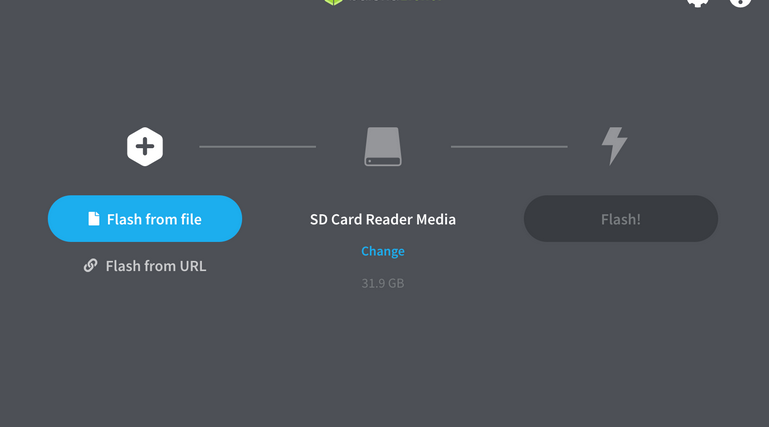
\includegraphics[width=0.75\textwidth]{imagenes/etcher.png}
	\caption{Interfaz de la aplicación Etcher}
\end{figure}

3. Una vez grabada la imagen, se ha de insertar la tarjeta SD en la Raspberry Pi, encenderla y proceder a la configuración básica como cualquier otro sistema operativo.\\

\section{Instalación y configuración del broker}
Como broker MQTT se ha elegido Mosquitto, aunque existen otras muchas alternativas\cite{ref28} como Cassandana, RabbitMQ, EMQ X, Apache ActiveMQ, etc.\\

Para instalar Mosquitto, usaremos el gestor de paquetes de Raspbian ejecutando los siguientes comandos:\\
\begin{lstlisting}[language=python]
	sudo apt update && sudo apt upgrade
	sudo apt install mosquitto mosquitto-clients
\end{lstlisting}

Si queremos que Mosquitto se lance automaticamente cuando arranque la raspberry, se ha ejecutar el siguiente comando para añadir el servicio de Mosquitto a la lista que se ejecuta nada mas arrancar:\\
\begin{lstlisting}[language=python]
	sudo systemctl enable mosquitto.service
\end{lstlisting}

\subsection{Probando Mosquitto}

Para probar que Mosquitto funciona correctamente, podemos usar el comando mosquitto\_sub para suscribirnos a un topic y el comando mosquitto\_pub para publicar en un topic.\\
\subsubsection{Suscribirse a un topic}
Con -h indicaremos la IP del broker al que nos queremos conectar, en este caso la IP de la raspberry pi. Con -t indicaremos el topic al que nos queremos suscribir.\\
\begin{lstlisting}[language=python]
mosquitto_sub -h 192.168.1.200 -t test
\end{lstlisting}

\subsubsection{Publicar a un topic}
Para publicar a un topic, al igual que parar subcribirnos, usaremos la opcion -h para indicar la IP del broker y la opción -t para indicar el topic al que queremos publicar. Pero además, se ha de añadir la opción -m con la que se indicará el mensaje que queremos publicar.\\

\begin{lstlisting}[language=python]
mosquitto_pub -h 192.168.1.200 -t test -m "this is a test message"
\end{lstlisting}

\begin{figure}[h!]
	\centering
	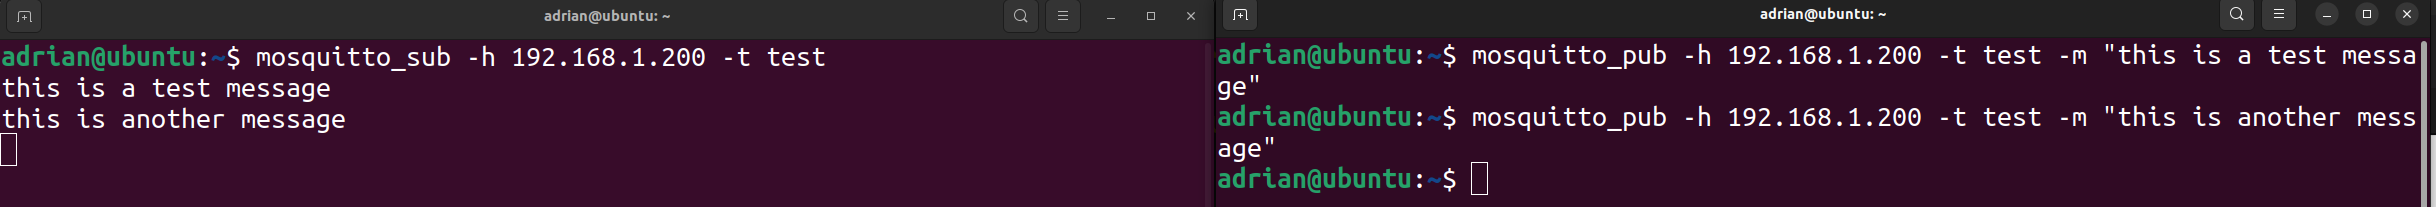
\includegraphics[width=1\textwidth]{imagenes/mqtt_test.png}
	\caption{Ejemplo de uso de Mosquitto}
\end{figure}

\end{titlepage}
